\begin{frame}{Signal Protocol}
    \framesubtitle{Il protocollo: X3DH}
    X3DH è stato sviluppato da OWS per supportare lo scambio asincrono delle chiavi. \cite{X3DH}\pause\newline
    Definizioni:
    \begin{itemize}
        \item Identity key: chiave pubblica\pause
        \item Ephemereal key: chiave utilizzabile una sola volta \pause
        \item Pre-keys: chiavi condivise col server prima dell'attivazione del protocollo\pause
        \item One-time pre-keys: insiemi di pre-keys condivisi col server prima dell'attivazione del protocollo. Il server condivide una chiave ogni volta che un utente vuole iniziare una conversazione e ne richiede un nuovo insieme quando stanno per finire\pause
        \item Signed pre-key: pre-key firmata con l'esponente dell'Identity key
    \end{itemize}

    \note{
        STANDARD DIFFIE-HELLMAN: Alice e Bob generano ognuno una chiave pubblica \textit{pk} basata su un generatore comune \textit{g} modulo \textit{m} e le proprie chiavi private (\textit{secret keys}) \textit{sk}. \\Dopodiché scambiano le chiavi pubbliche attraverso un canale (potenzialmente non sicuro) e da esse possono derivare una chiave segreta condivisa \textit{ssk}.
        \cite{diffiehellman}, \cite{diffiehellman2}
    }
\end{frame}

\begin{frame}{Signal Protocol}
    \framesubtitle{Il protocollo: X3DH}

    \begin{figure}
        \centering
        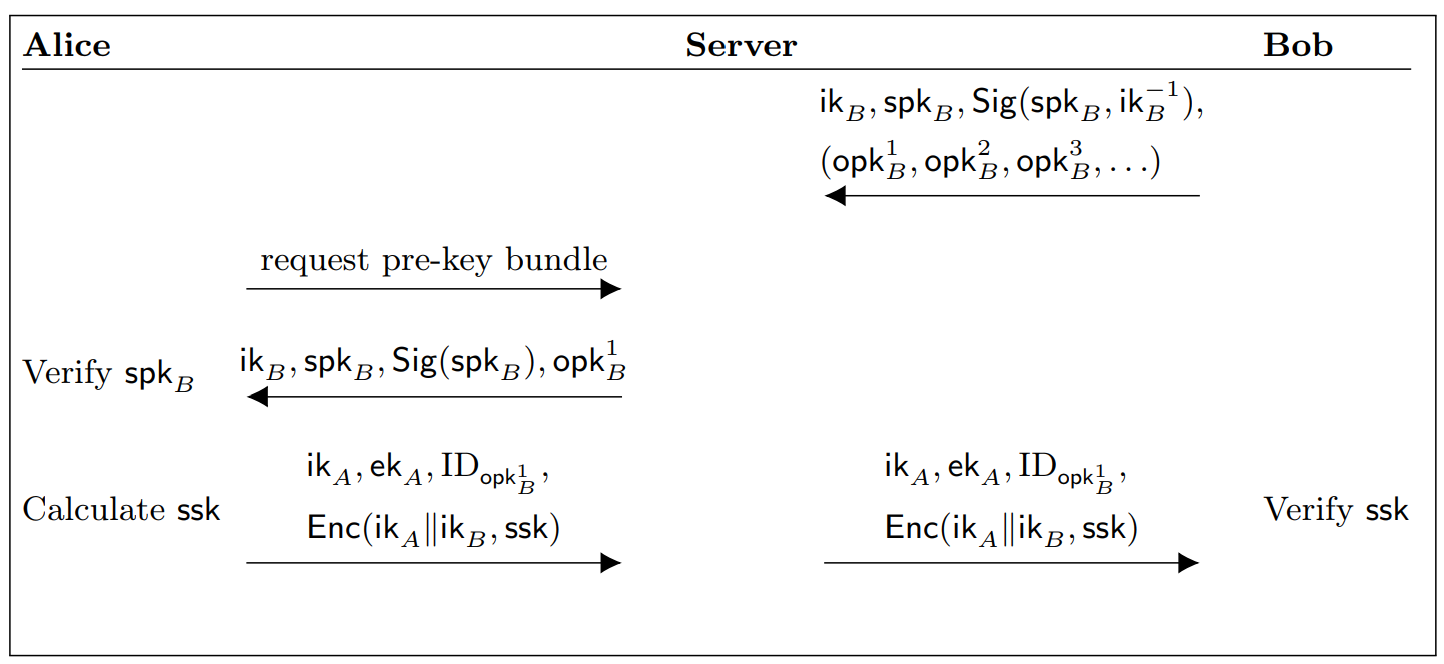
\includegraphics[width=.8\textwidth]{X3DH.png}
        \caption{Funzionamento di X3DH semplificato}
        \label{tag: X3DH simplified}
    \end{figure}

    \cite{VanDam}

    \note{
        Perché il protocollo possa funzionare offline ogni utente deve inviare le proprie chiavi pubbliche al server, inviando cioè \(ik, spk, Sig(spk, ik^{-1}\) e \((opk^1, opk^2, opk^3,...)\).\newline
        La \(ik\) va inviata una sola volta, la \(spk\) va rinnovata periodicamente.\newline
        Se Alice vuole iniziare una conversazione richiede al server \(ik_B\), \(spk_B\), \(Sig(spk_B, ik_B^{-1}\) e una delle one-time pre-keys \(opk_B^x\) di Bob. Il server poi elimina \(opk_B^x\). Una volta finite le \(opk_B\) ad Alice verranno inviate solo le altre chiavi senza \(opk_B\).\newline
        Ricevute le chiavi Alice verifica la firma di \(spk_B\) e se va a buon fine genera una coppia di chiavi effimere; poi calcola la \(ssk\) usando una Key Derivation Function (KDF). Alla fine cancella \(ek_A^{-1}\) e tutti i valori \(k_i\) generati.\newline
        N.B. \(DH(x, y)\) è una funzione DH su curva ellittica che calcola una \(ssk\) basandosi su due chiavi, mentre \(KDF(x)\) è una funzione basata su  RFC5869  \cite{KDF}.\newline
        Alice invia un messaggio iniziale a Bob contenente \(ik_A\), \(ek_A\), \(ID_{opk_B^x}\) (per fargli sapere quale \(opk_B^x\) ha usato) e \(Enc(ik_A || ik_B, ssk)\).\newline
        Bob riceve il messaggio e calcola la \(ssk\) nello stesso modo di Alice. Bob decritta il messaggio inviato da Alice e controlla se il valore di \(ssk\) è corretto e in questo caso cancella la \(opk\) utilizzata.\newline
        Alice e Bob possono ora riutilizzare la stessa \(ssk\) per messaggi futuri oppure usare chiavi da essa derivate.
        \cite{VanDam}
    }
\end{frame}
